\documentclass{beamer}
\usepackage{caption}
\usepackage{subcaption}

\title{Conformance Checking Using Embeddings and its Applicability in the Internet of Things}
\author{Jan Kruska}
\date{\today}

\begin{document}
	
	\frame{\titlepage}
	
	\begin{frame}
		\frametitle{Table of Contents}
		\tableofcontents
	\end{frame}
	\section{Conformance Checking}
	\begin{frame}
		\frametitle{Conformance Checking}
	\end{frame}
	
	\section{Embeddings}
	\begin{frame}
		\frametitle{Embeddings}
	\end{frame}
	
	
	\begin{frame}
		\frametitle{\emph{act2vec} \& \emph{trace2vec}}
	\end{frame}
	
	\section{Experiments}
	\begin{frame}
		\frametitle{Setup}
		Random trees were generated using pm4py and the following configurations:
		
		\begin{tabular}{lll}
			Min & Mode & Max \\
			5 & 10 & 15 \\
			10 & 20 & 30 \\
			15 & 30 & 45 \\
		\end{tabular}
		\begin{tabular}{llll}
			Sequence & Parallel & Choice & Loop \\
			0.75 & 0.25 & 0 & 0 \\
			0.75 & 0 & 0.25 & 0 \\
			0.5 & 0.25 & 0.25 & 0 \\
			0.25 & 0.25 & 0.25 & 0.25 \\
		\end{tabular}
		
		Using these parameters $3\times4=12$ trees were generated.
	\end{frame}
	\begin{frame}
		\frametitle{Example tree}
		\begin{figure}
			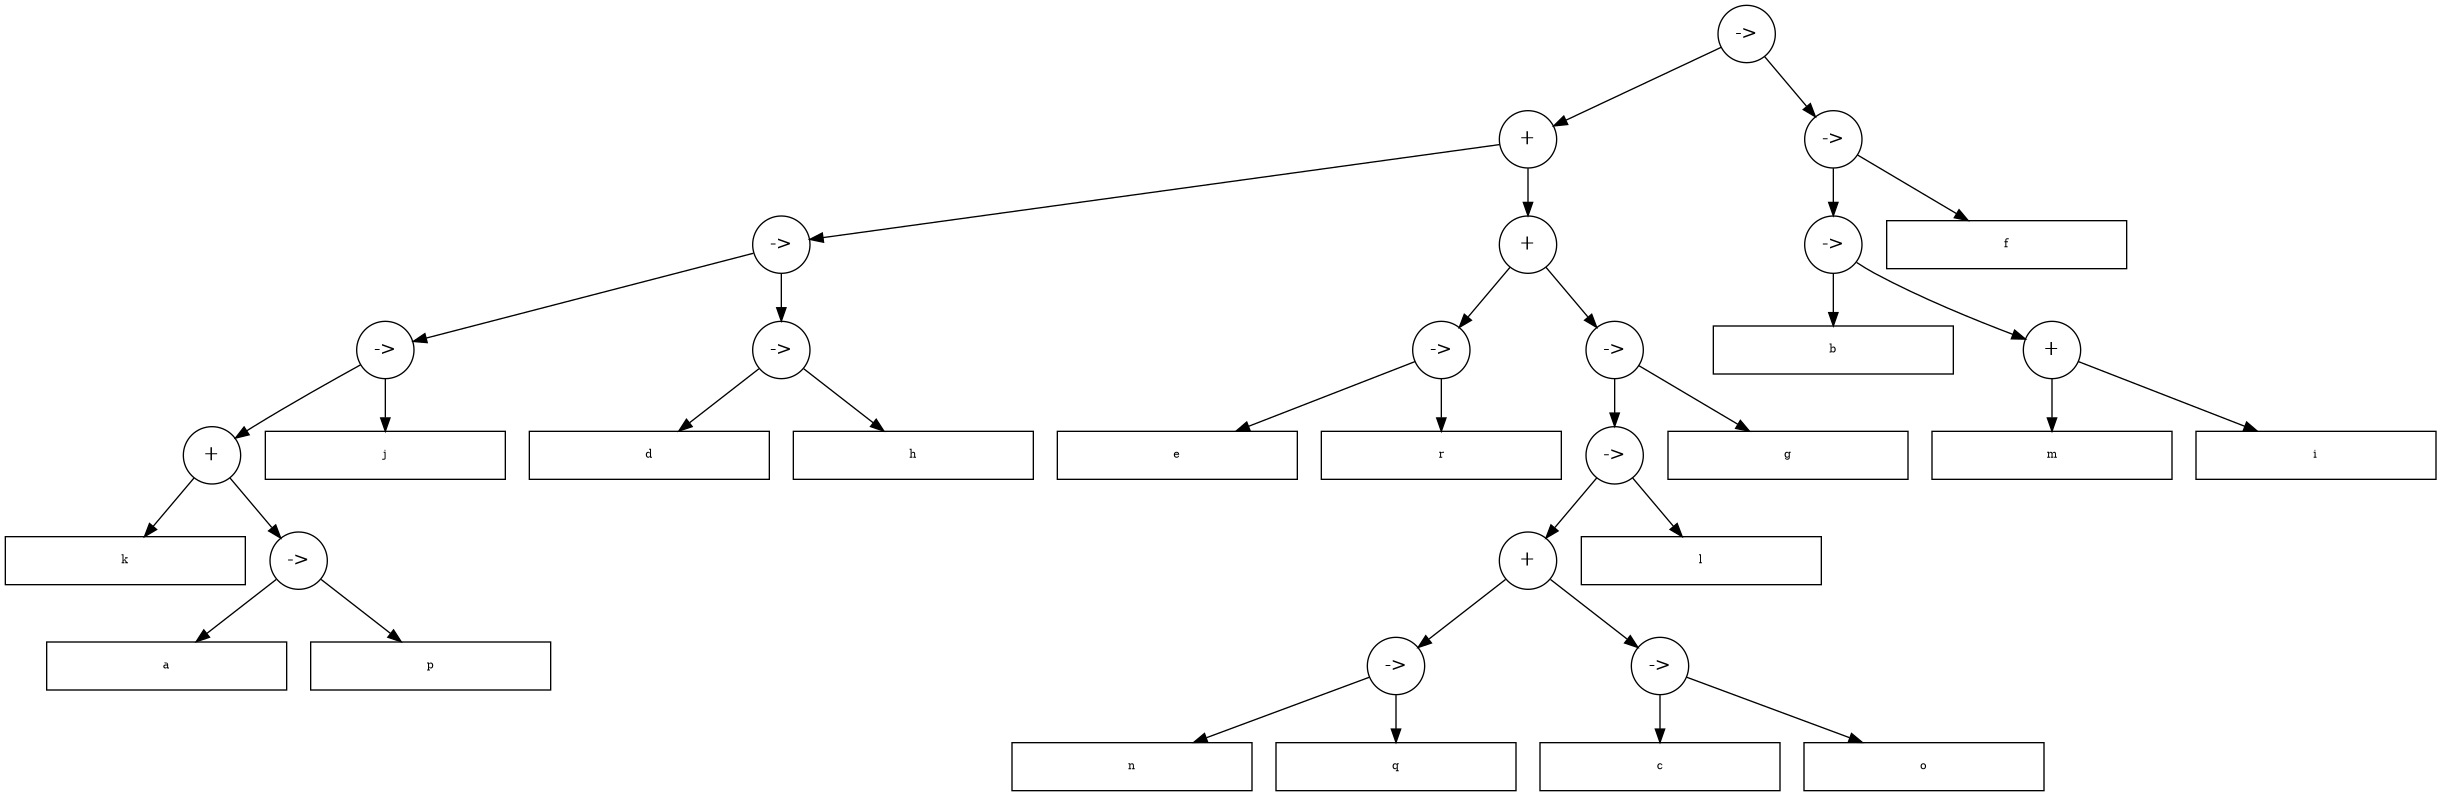
\includegraphics[width=1\textwidth]{figures/process-tree}
			\caption{A process tree generated by pm4py using parameters: Min 15, Mode 30, Max 45, sequence 0.75, parallel 0.25. }
			\label{fig:process-tree}
		\end{figure}
	\end{frame}
	
	\begin{frame}
		\frametitle{Noise}
		\begin{figure}
			\centering
			\begin{subfigure}[b]{0.49\textwidth}
				\centering
				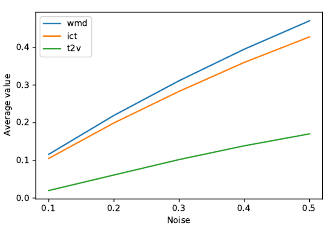
\includegraphics[width=\textwidth]{figures/noise-first}
				\caption{Average of first noise experiment (Varying trace percentage).}
				\label{fig:noise-first}
			\end{subfigure}
			\hfill
			\begin{subfigure}[b]{0.49\textwidth}
				\centering
				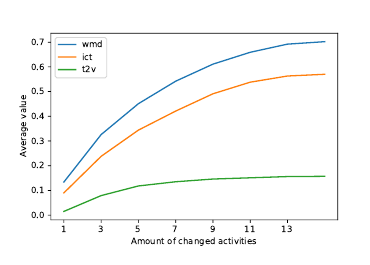
\includegraphics[width=\textwidth]{figures/noise-second}
				\caption{Average of second noise experiment (Varying amount of noise applied to trace).}
				\label{fig:noise-second}
			\end{subfigure}
		\end{figure}
	\end{frame}
	
	
	\begin{frame}
		\frametitle{Discovery}
		\begin{figure}
			\centering
			\begin{subfigure}[b]{0.49\textwidth}
				\centering
				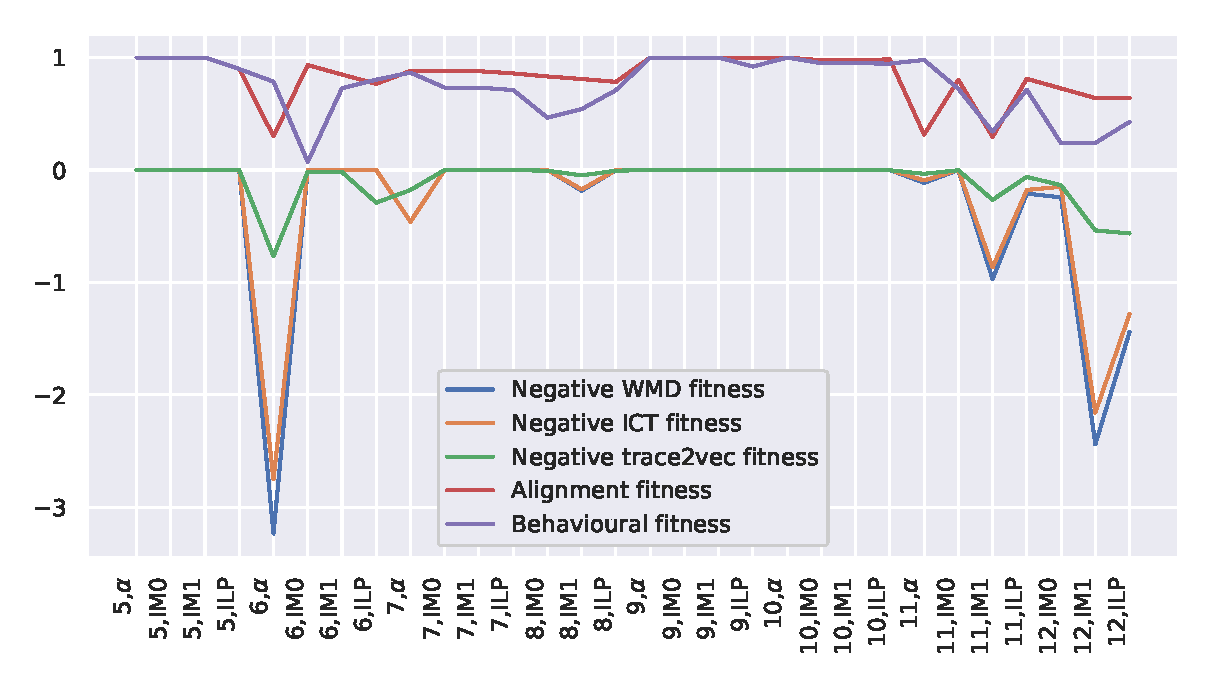
\includegraphics[width=\textwidth]{figures/fitness}
				\caption{Fitness}
				\label{fig:fitness}
			\end{subfigure}
			\hfill
			\begin{subfigure}[b]{0.49\textwidth}
				\centering
				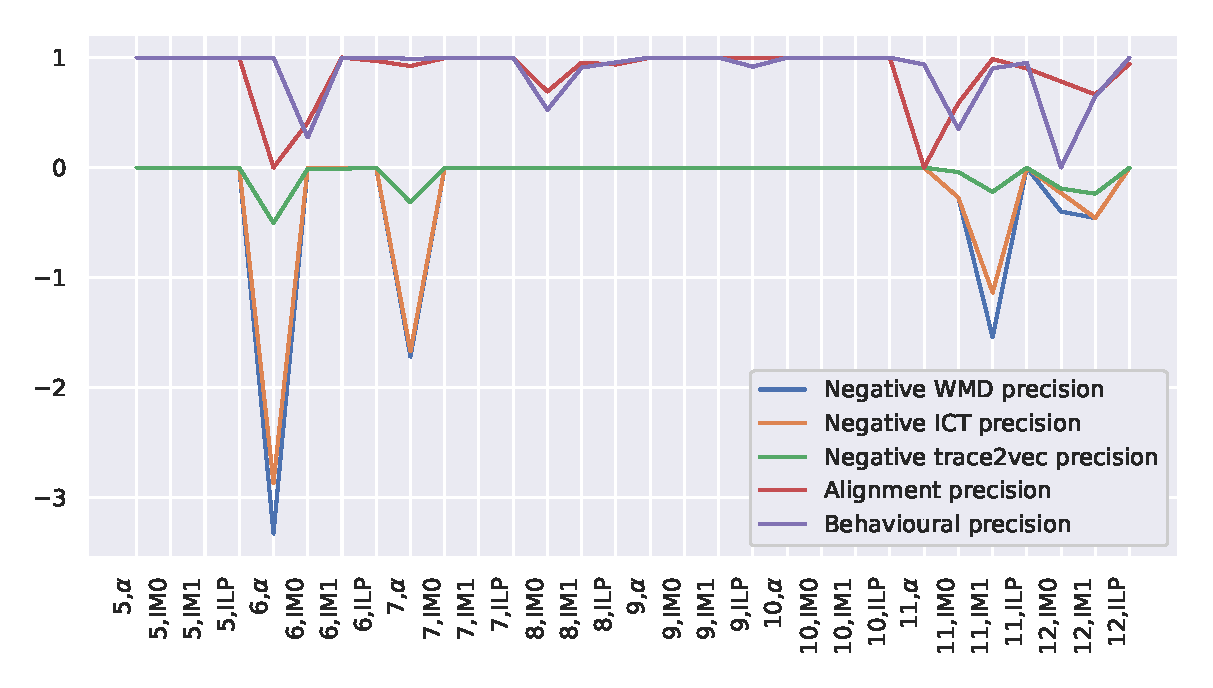
\includegraphics[width=\textwidth]{figures/precision}
				\caption{Precision}
				\label{fig:precision}
			\end{subfigure}
			\caption{Fitness and Precision for different tree, discovery technique pairings for the three proposed techniques as well as the two verification techniques.}
			\label{fig:discovery}
		\end{figure}
	\end{frame}
	
	\begin{frame}
		\frametitle{Discovery}
		\begin{itemize}
			\item Measures for proposed methods are not proper fitness metrics, so careful with quantitative analyses!
			\item 
		\end{itemize}
	\end{frame}
	
	
	\begin{frame}
		\frametitle{Scalability}
		\begin{figure}
			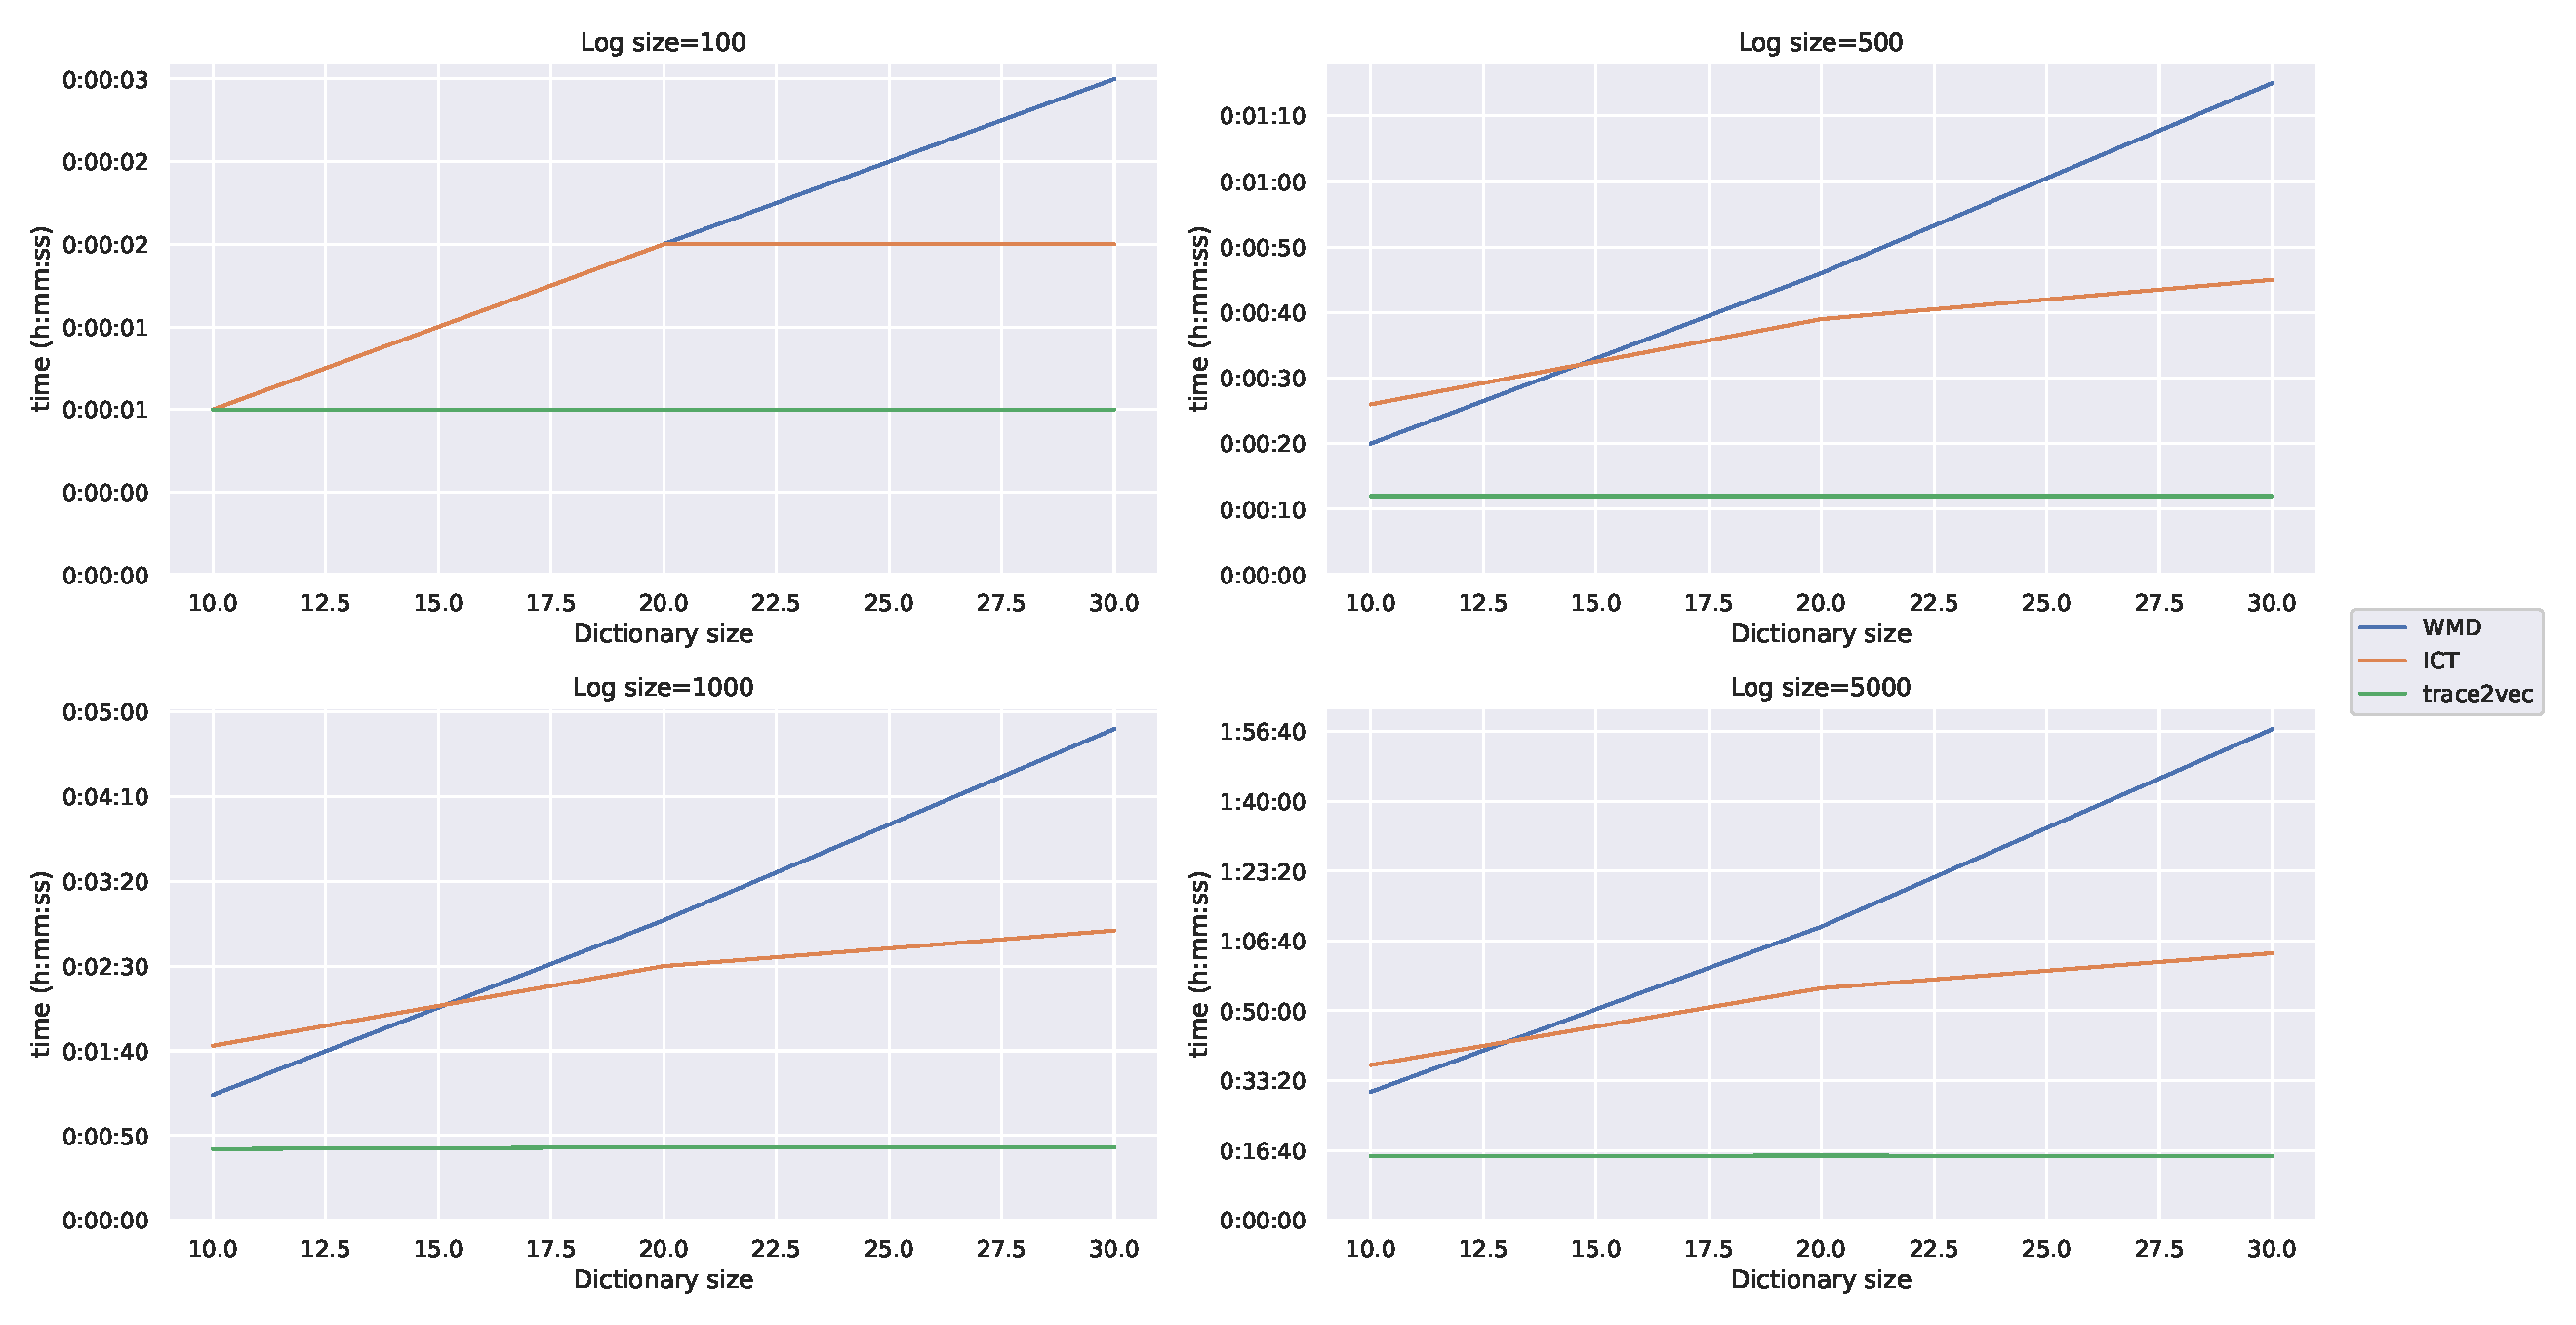
\includegraphics[width=1\textwidth]{figures/scaling}
			\caption{Runtimes for all three methods for varying sizes of logs and dictionaries.}
			\label{fig:scalability}
		\end{figure}
	\end{frame}
	
	\section{Internet of Things}
	\begin{frame}
		\frametitle{Challenges}
		\begin{itemize}
			\item log-comparison method. Performance dependent on model complexity. How many traces are needed to describe the model sufficiently well.
		\end{itemize}
	\end{frame}
	
	\begin{frame}
		\frametitle{Benefits}
		\begin{itemize}
			\item Better performance, and especially better scaling w.r.t. number of activities and trace length.
			\item Embeddings have other advantages, no more binary activity equality, could allow for more fine grained conformance.
		\end{itemize}
	\end{frame}
	
\end{document}